
\documentclass[11pt]{article}
 
\usepackage[margin=1in]{geometry} 
\usepackage{amsmath,amsthm,amssymb}
\usepackage{graphicx} 
\usepackage{blkarray}
\usepackage{amsmath}




\newcommand{\N}{\mathbb{N}}
\newcommand{\Z}{\mathbb{Z}}
 
\newenvironment{problem}[2][Problem]{\begin{trivlist}
\item[\hskip \labelsep {\bfseries #1}\hskip \labelsep {\bfseries #2.}]}{\end{trivlist}}
\newenvironment{lemma}[2][Lemma]{\begin{trivlist}
\item[\hskip \labelsep {\bfseries #1}\hskip \labelsep {\bfseries #2.}]}{\end{trivlist}}
\newenvironment{exercise}[2][Exercise]{\begin{trivlist}
\item[\hskip \labelsep {\bfseries #1}\hskip \labelsep {\bfseries #2.}]}{\end{trivlist}}

\newenvironment{question}[2][Question]{\begin{trivlist}
\item[\hskip \labelsep {\bfseries #1}\hskip \labelsep {\bfseries #2.}]}{\end{trivlist}}
\newenvironment{corollary}[2][Corollary]{\begin{trivlist}
\item[\hskip \labelsep {\bfseries #1}\hskip \labelsep {\bfseries #2.}]}{\end{trivlist}}

\usepackage{indentfirst}
\linespread{1.2}     % 调整间距
\setlength{\parindent}{0pt}

\begin{document}

 
% --------------------------------------------------------------
%                         Start here
% --------------------------------------------------------------
 
\title{Homework 9 DS-GA 1002 }%replace X with the appropriate number
\author{Yuhao Zhao\\ %replace with your name
Yz3085} %if necessary, replace with your course title
 
\maketitle
\begin{problem}{1}
\end{problem}
a) False, The projection on a subspace can be any vector in the space not necessarily the orthogonal projection. \\
For example, v = (1,1,1),  S is the x,y plane,  $span\{\begin{bmatrix}
	1\\0\\0
	\end{bmatrix},\begin{bmatrix}
	0\\1\\0
	\end{bmatrix} \}$\\ The projection of v onto S can be any vector in the S. not necessarily the orthogonal projection (1,1,0)\\
	
b)\\   (i) If the inner product is defined on finite dimension space with dimension n, it's true (ie. all subspaces of a finite dimension vector space are closed):\\

proof:\\ if $V \in S,\text{for}$ $ \forall W \in S^{\perp}, <V,W> = 0$, by definition of complement, $V \in $the complement of $S^{\perp}$, therefore $V\in  (S^{\perp})^{\perp}$\\
if $V \in (S^{\perp})^{\perp},$ assume $V \notin S$, let $\{u_1,...u_p\}$ be an orthogonal basis of S, and $\{w_1,...w_q\}$  be an orthogonal basis of $S^{\perp}$, we know that p+q = n.\\ Assume $V\notin S, \{u_1,...u_p,V\}$ are linearly independent, and $V \perp\{w_1,...w_q\} $\\ therefore, $\{u_1,...u_p,V,w_1,...w_q\}$ are linearly independent. This is contradict to the fact that n dim space can't have  n+1 linearly independent vectors.Therefore, V $\in S$\\
Therefore, $S = (S^{\perp})^{\perp}$\\

(ii) In a infinite Hilbert space, the subspace can be open, the orthogonal complement is close. $\bar{S} = (S^{\perp})^{\perp}$ \\
In a Banach space, $i\bar{S} = (S^{\perp})^{\perp}$, so the statement is false.\\

c) FALSE. if the initial value is orthogonal to $v_1$, for example, if the initial vector is one of the eigenvectors, no matter how many times we apply the matrix, the result we get will be the initial vector.\\
Let A = $\begin{bmatrix}
1& 2\\2 &1
\end{bmatrix}$, the eigenvalues are 3 and -1, with corresponding eigenvectors  $V_1 = \begin{bmatrix}
1\\1
\end{bmatrix},V_2 = \begin{bmatrix}
1\\-1
\end{bmatrix}$  If we set the initial vector to be $V_2 = \begin{bmatrix}
1\\-1
\end{bmatrix}$, $A^{k}V_2 = V_2$ and wont converge to $V_1$\\

\begin{problem}{2}
\end{problem}
a) Let $V_1$ be $Y_1$, then $||V_1|| = E(V_1^2) = E(B^2 +M^2 +2BM)=3\sigma^2 + 2E(BM)$\\ $B, M$ are uncorrelated, $E(BM)-E(B)E(M) = 0, E(B) =E(M) = 0$,$E(BM) = 0$.\\ Therefore $||V_1|| = \sqrt{4\sigma^2} = 2\sigma$ , $e_1 = \frac{V_1}{||V_1||}= \frac{Y_1}{2\sigma}$\\

$V_2 = Y_2 - <Y_2,e_1>e_1 = Y_2 - E(Y_2e_1)e_1,  E((M+N)Y_1) = 3\sigma^2$ \\
$V_2 = Y_2 - \frac{3\sigma^2}{2\sigma}\frac{Y_1}{2\sigma} = Y_2 - \frac{3}{4}Y_1$\\
$||V_2||^2= E(Y_2^2 + \frac{9}{16} Y_1^2-\frac{3}{2}Y_1Y_2) = 4\sigma^2 + \frac{9}{16}\times 4\sigma^2 - \frac{3}{2}\times 3 \sigma^2 = \frac{7}{4}\sigma^2$\\
Therefore, $e_2 = \frac{V_2}{||V_2||} = \frac{Y_2 - \frac{3}{4}Y_1}{\frac{\sqrt{7}}{2}\sigma}$\\
$\{e_1,e_2\}$ is an orthonormal basis for span$\{Y_1,Y_2\}$ \\

b) Since B, $Y_1, Y_2$ are all zero mean random variables, the best linear estimator of B given $Y_1, Y_2$ won't have a constant term. \\
The orthogonal projection of B onto the subspace S spanned by $\{Y_1,Y_2\}$ is the closest vector to B that belongs to S in terms of the norm induced by the inner product. We use the Expectation as the inner product, therefore, the orthogonal projection onto $\{Y_1,Y_2\}$ (or $\{e_1,e_2\}$) will minimize the MSE.\\
$g_{LMMSE}(Y_1,Y_2) =P_S(B) = P_{span\{e_1,e_2\}}(B) = <e_1,B>e_1+ <e_2,B>e_2$\\
$= E(\frac{Y_1}{2\sigma}B)\frac{Y_1}{2\sigma} +E(B\frac{Y_2 - \frac{3}{4}Y_1}{\frac{\sqrt{7}}{2}\sigma})\frac{Y_2 - \frac{3}{4}Y_1}{\frac{\sqrt{7}}{2}\sigma} \\
= \frac{\sigma^2}{2\sigma} \frac{Y_1}{2\sigma}- \frac{3}{4}\times \frac{4}{7} \times(Y_2 - \frac{3}{4}Y_1)\\
= \frac{1}{4}Y_1 - \frac{3}{4}Y_2 + \frac{9}{28}Y_1\\ = \frac{4}{7}Y_1 - \frac{3}{7}Y_2$\\

$Y_2$ is the observed approximated heartbeat of the mother, $Y_1$ is the observation of sum heartbeat of the mom and baby. Therefore, once we have the  the mother's approximate heartbeat $Y_1$ and the observation of sum heartbeat $Y_2$, the best linear estimation of the baby's heartbeat will be $\frac{4}{7}Y_1 - \frac{3}{7}Y_2$\\
\pagebreak

 \begin{problem}{3}
 \end{problem}
a)Denote h as healthy and i as ill, The transition matrix is  \[P = 
\begin{blockarray}{ccc}
&\text{h} & \text{i}\\
\begin{block}{c(cc)}
\text{h} & 0.9  &0.1 \\
\text{i}  & 0.2 &0.8 \\
\end{block}
\end{blockarray}
\]\\ The stationary distribution $\pi$ is $\pi P = \pi, \pi(P-I)=0$, we need to solve, $(P-I)'\pi' = 0$\\
$\pi =  (\frac{2}{3},\frac{1}{3})$\\
Therefore, if we assume the health condition of Bob today only depends on the condition yesterday, and the Markov chain has converged to the stationary,  the probability of Bob being ill is $\frac{1}{3}$\\

b) Given Bob ill today $g_{MAP} = \underset{H \in \{h, i\}} {\mathrm{Argmin}} ~ \pi_H P^3 \begin{bmatrix}
0\\1
\end{bmatrix} $ where, $\pi_h = (1,0), \pi_i = (0,1)$\\
$H =i, \quad (0,1) P^3\begin{bmatrix} 0\\1 \end{bmatrix} = 0.562$ \\
$H = h, \quad (1,0) P^3\begin{bmatrix} 0\\1 \end{bmatrix} = 0.219$\\
Therefore, The gap estimate is ill\\

\begin{problem}{4}
\end{problem}
a) 

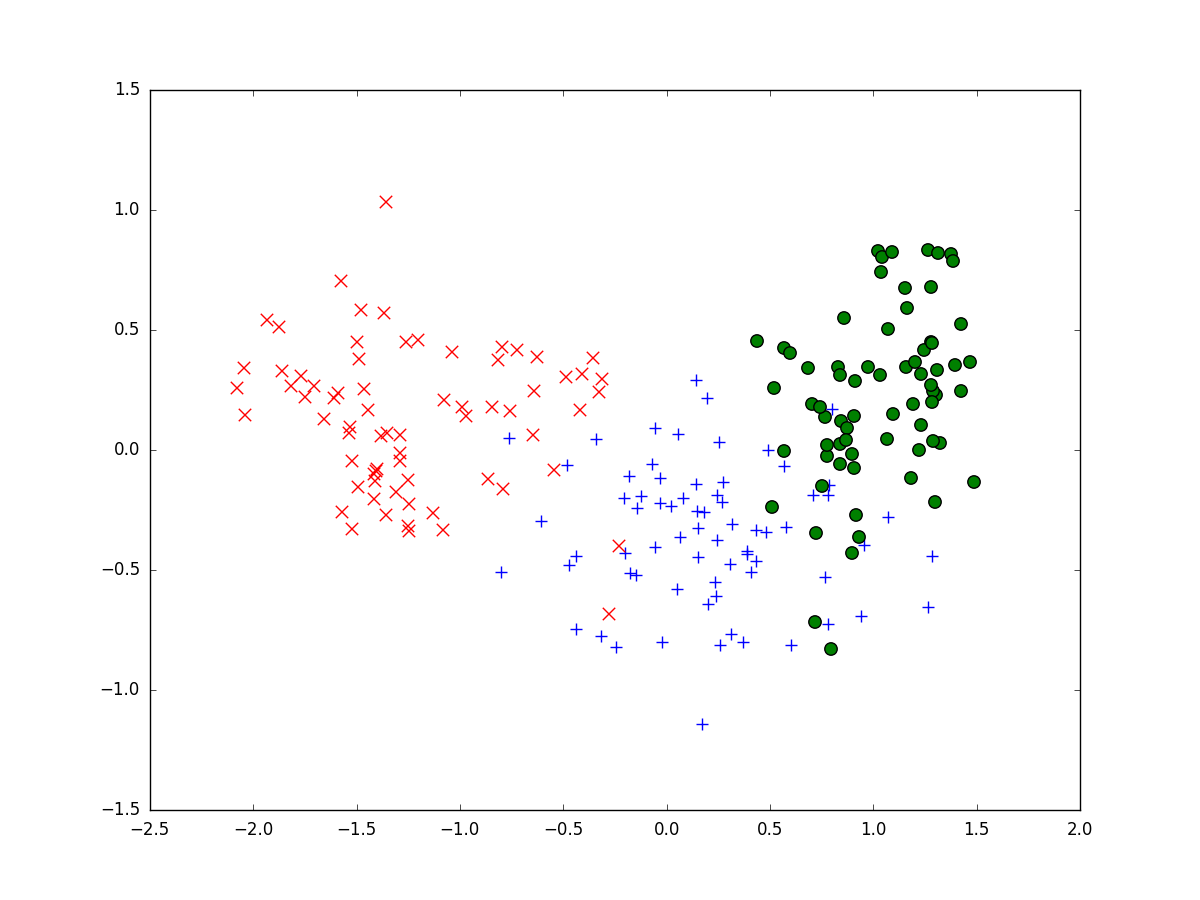
\includegraphics[width = 5in]{f} \\ 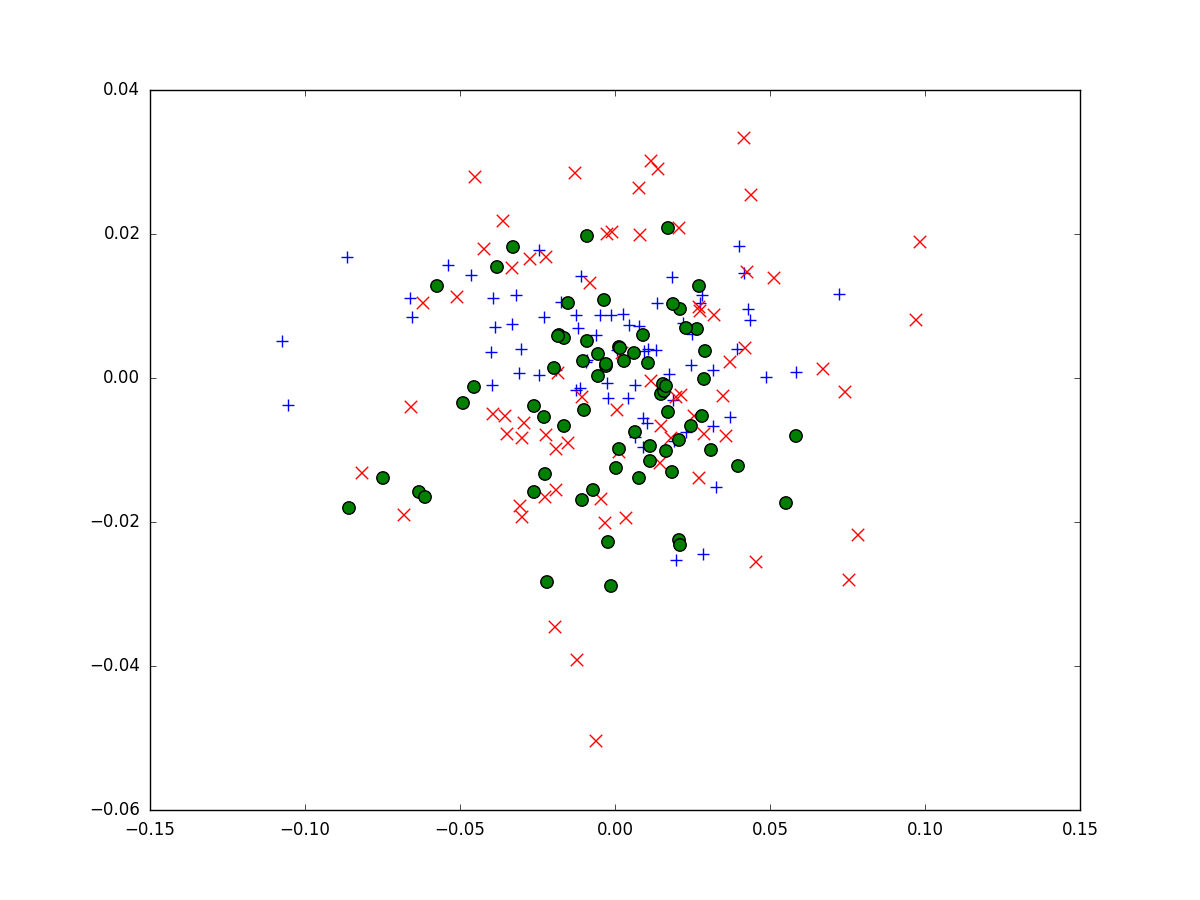
\includegraphics[width = 5in]{l}

The energy of the projection of the data points onto different
directions in the ambient space reflects the variation of the dataset along those directions. The projection on the first two PC preserves the most energy and greastest variance among the two directions, and it shows clear cluster behavior. The projection on the last two PC preserves the least variance, and the projections of points are mixed. \\

b) 
To predict the seed type, we can project the seeds vector onto the first two PCs we calculated and use KNN to decide the test label of the seeds.\\
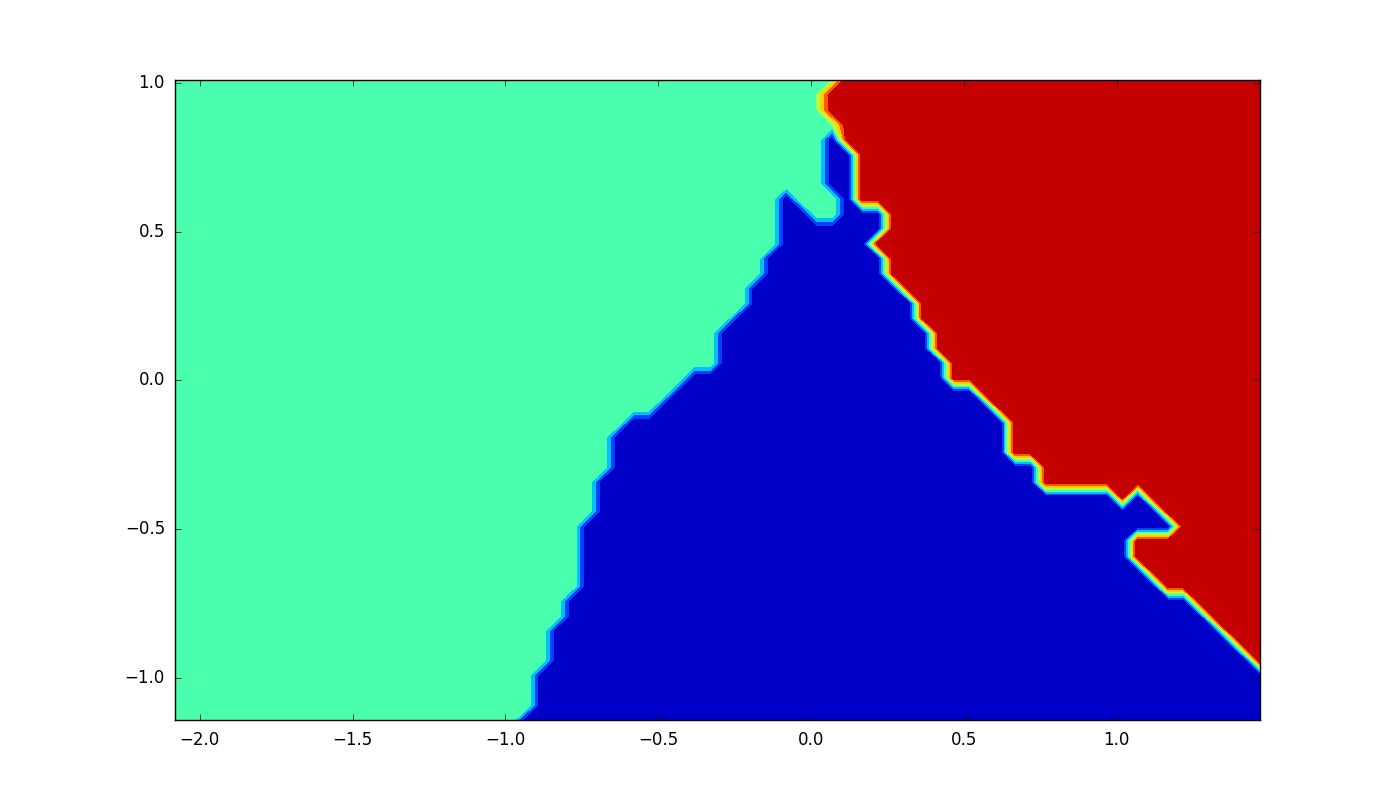
\includegraphics[width = 5in]{knn}

The above plots shows the decision region classified by the knn method. In particular, if the projection of the point lies in the blue/red/green region, it should be classified as type 1/2/3.
\end{document}